\documentclass{article}
\usepackage{graphicx}
\usepackage{amsmath}
\usepackage{pgfplots}
\usepackage{tikz}
\usepackage{txfonts}
\usepackage{physics}
\usepackage{hyperref}
\usepackage[a4paper, top=1cm, bottom=2cm, left=2cm, right=2cm, includehead, includefoot]{geometry}
\pgfplotsset{compat=1.18}

\begin{document}
\noindent
Physics 4A - Classical Mechanics \hfill Prof. Roger King

\noindent\rule{\textwidth}{0.4pt}

\begin{center}
    \textbf{\LARGE Chapter 3 - Vectors} \\
    \vspace{12pt}
    \large Aaron W. Tarajos \\
    \textit{\today}
\end{center}

\noindent\rule{\textwidth}{0.4pt}

\section*{3.1 Vectors and Their Components}
\subsection*{key ideas}
\begin{itemize}
	\item Scalars consist of only magnitude and are subject to the ordinary rules of algebra.
	Vectors consist of magnitude and direction and are subject to the rules of vector algebra.
	\item Two vectors $\vec{a}$ and $\vec{b}$ can be added geometrically by drawing them at common scales and place them head to tail.
	The vector $\vec{s}$ that connects the head and the tail is the summed vector.
	To subtract a vector switch the direction of the one you are subtracting and then proceed as if you were adding them.
	\item The scalar components, $(a_x, a_y, a_z, \dots)$, of a vector $\vec{a}$ are found by dropping perpendicular lines from the ends of
	$\vec{a}$ onto the coordinate axes. In two dimensions, the components are given by;
	\[
		a_x = a \cos{\theta} \quad \text{and} \quad a_y = a \sin{\theta}
	\]
	and the magnitude and orientation by;
	\[
		a = \sqrt{a_x^2 + a_y^2} \quad \text{and} \quad \tan(\theta) = \frac{a_y}{a_x}
	\]
\end{itemize}

\subsection*{3.1.1 Vectors and Scalars}
\textbf{Motion:}
	A particle moving along a straight line can move in two directions, which can be represented as positive or negative motion.
	For a particle moving in three dimensions, using just a plus or minus sign is insufficient; vectors are needed to represent both direction and magnitude.
\vspace{12pt}\\
\textbf{Vectors:}
    A vector has both magnitude and direction and follows specific rules for combination.
    Vector quantities: These are physical quantities that have both magnitude and direction, such as displacement, velocity, and acceleration.
\vspace{12pt}\\
\textbf{Scalars:}
    Physical quantities that do not have a direction, like temperature, pressure, energy, mass, and time.
    Scalars are handled using regular algebra, and a single value (with a sign) specifies them.
\vspace{12pt}\\
\textbf{Displacement:}
    The simplest vector quantity, which represents a change in position.
    A vector representing displacement is called a displacement vector.
    The arrow from point A to B shows displacement, and vectors with the same magnitude and direction (even if shifted) represent the same displacement.

\subsection*{3.1.2 Adding Vectors Geometrically}
Given a particle that moves from A to B and then B to C.
We represent the overall displacement, regardless of the path taken, as two displacement vectors AB and BC.
The net displacement is the \textbf{vector sum} AC.
\begin{center}
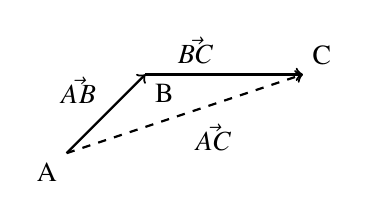
\begin{tikzpicture}[scale=1]
    % Points
    \coordinate (A) at (0,0);
    \coordinate (B) at (1,1);
    \coordinate (C) at (3,1);

    % Vectors
    \draw[thick,->] (A) -- (B) node[midway,above left] {$\vec{AB}$};
    \draw[thick,->] (B) -- (C) node[midway,above left] {$\vec{BC}$};
    \draw[thick,dashed,->] (A) -- (C) node[midway,below right] {$\vec{AC}$};

    % Points Labels
    \node[below left] at (A) {A};
    \node[below right] at (B) {B};
    \node[above right] at (C) {C};
\end{tikzpicture}
\end{center}
The order of the addition does not matter. This is the commutative law;
\[
	\vec{a} + \vec{b} = \vec{b} + \vec{a}
\]
While adding two vectors works the way someone may intuitively guess, subtracting is a little different than scalar subtraction.
\[
	\vec{d} = \vec{a} - \vec{b} = \vec{a} + (-\vec{b})
\]
The vector being subtracted is changed to the opposite direction and then added.

\subsection*{3.1.3 Component Vectors}
\subsubsection*{Vector Components}
A \textit{component} of a vector is the projection of the vector on an axis. To find the projection of a vector along an axis, we draw perpendicular lines from the two ends of the vector to the axis.
The projection of a vector on the $x$ axis is its $x$ component, and similarly the projection on the $y$ axis is the $y$ component.
This process of finding the components of a vector is called \textit{resolving} the vector.
A component of a vector has the same direction (along an axis) as the vector.
If we were to reverse vector $\vec{a}$, then both components would be negative, and their arrowheads would point toward the negative $x$ and $y$ directions.

\subsubsection*{Finding the Components}
We can find the components of $\vec{a}$ geometrically from the right triangle:
\[
a_x = a \cos \theta \quad \text{and} \quad a_y = a \sin \theta
\]
where $\theta$ is the angle that vector $\vec{a}$ makes with the positive $x$ axis, and $a$ is the magnitude of $\vec{a}$.
We arrange those components head to tail, and then complete a right triangle with the vector forming the hypotenuse, from the tail of one component to the head of the other.

\subsubsection*{Component Notation vs Magnitude-Angle Notation}
Once a vector has been resolved into its components along a set of axes, the components themselves can be used in place of the vector.
It can also be given by its components $a_x$ and $a_y$. Both pairs of values contain the same information. If we know a vector in component notation ($a_x$ and $a_y$) and want it in magnitude-angle notation ($a$ and $\theta$), we can use the equations:
\[
a = \sqrt{a_x^2 + a_y^2} \quad \text{and} \quad \tan \theta = \frac{a_y}{a_x}
\]

\subsubsection*{Three-Dimensional Vectors}
In the more general three-dimensional case, we need a magnitude and two angles (say, $a$, $\theta$, and $\phi$) or three components ($a_x$, $a_y$, and $a_z$) to fully specify a vector.

\section*{3.2 Unit Vectors, Adding Vectors By Components}
\subsection*{key ideas}
\begin{itemize}
	\item Unit vectors $\hat{i}$, $\hat{j}$, and $\hat{k}$ are the base unit vectors with a magnitude of 1 and directed in the positive direction of the $x$, $y$, and $z$ axes respectively.
	\item We write a vector $\vec{a}$ as

	\[
		\vec{a} = a_x \hat{i} + a_y \hat{j} + a_z \hat{k}
	\]
	\item $a_x$, $a_y$, $a_z$, are the scalar components that multiply the unit vectors to create $\vec{a}$
\end{itemize}
The unit vectors are used as base vectors to point in a particular direction.
The standard unit vectors are $\hat{i}$, $\hat{j}$, and $\hat{k}$ for the $x$, $y$, and $z$ axes respectively.
These vectors are orthogonal to eachother.
These are the most common unit vectors but others may be defined for some specific purpose. Sometimes $\hat{r}$ is used as a general case unit vector.\vspace{12pt} \\
Unit vector notation is particularly useful for vector algebra because we simply perform algebraic operations on the respective scalar components.
For example, with two vectors $\vec{a}$ and $\vec{b}$ that sum to create $\vec{r}$ we have;
\[
	\va r = \left(a_x b_x\right)\hat{i} + \left(a_y b_y\right)\hat{j}
\]

\section*{3.3 Multiplying Vectors}
\section*{Key Ideas}
\begin{itemize}
    \item \textbf{Scalar (Dot) Product}: The scalar product of two vectors $\vec{a}$ and $\vec{b}$ gives a scalar value and is calculated as:
    \[
    \vec{a} \cdot \vec{b} = ab \cos \theta
    \]
    where $a$ and $b$ are the magnitudes of the vectors and $\theta$ is the angle between them.
    \item \textbf{Vector (Cross) Product}: The vector product of two vectors $\vec{a}$ and $\vec{b}$ results in a vector that is perpendicular to both and is given by:
    \[
    \vec{a} \times \vec{b} = ab \sin \theta \hat{n}
    \]
    where $\hat{n}$ is a unit vector perpendicular to both $\vec{a}$ and $\vec{b}$.
    \item \textbf{Applications}: The dot product is used in finding the work done by a force, while the cross product is essential in calculating torque and angular momentum.
\end{itemize}

\subsection*{Scalar (Dot) Product}
The scalar product (or dot product) of two vectors results in a scalar quantity. For two vectors $\vec{a}$ and $\vec{b}$, the dot product is defined as:
\[
\vec{a} \cdot \vec{b} = ab \cos \theta
\]
where $a$ and $b$ are the magnitudes of the vectors, and $\theta$ is the angle between them. The scalar product can also be expressed in terms of components:
\[
\vec{a} \cdot \vec{b} = a_x b_x + a_y b_y + a_z b_z
\]
This product is useful in calculating physical quantities like work, which is given by the product of force and displacement along the same direction:
\[
W = \vec{F} \cdot \vec{d}
\]

\subsection*{Vector (Cross) Product}
The vector product (or cross product) of two vectors results in a vector. The cross product of vectors $\vec{a}$ and $\vec{b}$ is defined as:
\[
\vec{a} \times \vec{b} = ab \sin \theta \hat{n}
\]
where $\hat{n}$ is a unit vector perpendicular to both $\vec{a}$ and $\vec{b}$, and $\theta$ is the angle between them. The direction of $\hat{n}$ is determined by the right-hand rule. In component form, the vector product is:
\[
\vec{a} \times \vec{b} = (a_y b_z - a_z b_y) \hat{i} + (a_z b_x - a_x b_z) \hat{j} + (a_x b_y - a_y b_x) \hat{k}
\]
The vector product is used in calculating torque, which is the product of a force and the perpendicular distance from the point of rotation:
\[
\vec{\tau} = \vec{r} \times \vec{F}
\]

\subsection*{Applications in Physics}
The scalar product finds its applications in work, where the projection of force in the direction of motion is essential. The vector product is crucial in angular mechanics, especially in calculating quantities like torque and angular momentum. For example, torque is the vector product of the position vector $\vec{r}$ and force $\vec{F}$, given by:
\[
\vec{\tau} = \vec{r} \times \vec{F}
\]
The angular momentum $\vec{L}$ of a particle is similarly the vector product of the position vector $\vec{r}$ and linear momentum $\vec{p}$:
\[
\vec{L} = \vec{r} \times \vec{p}
\]



\end{document}
